\subsection{pinhole camera model}
In the junior high school physics class, we may have seen a candle projection experiment: a lit candle is placed in front of a black box, and the light of the candle is projected through a small hole in the dark box on the rear plane of the black box, and An inverted candle image is formed on this plane. In this process, the small hole model is able to project a candle in a three-dimensional world onto a two-dimensional imaging plane. For the same reason, we can use this simple model to explain the imaging process of the camera, as shown in \autoref{fig:cameraModel}.

\begin{figure}[!ht]
	\centering
	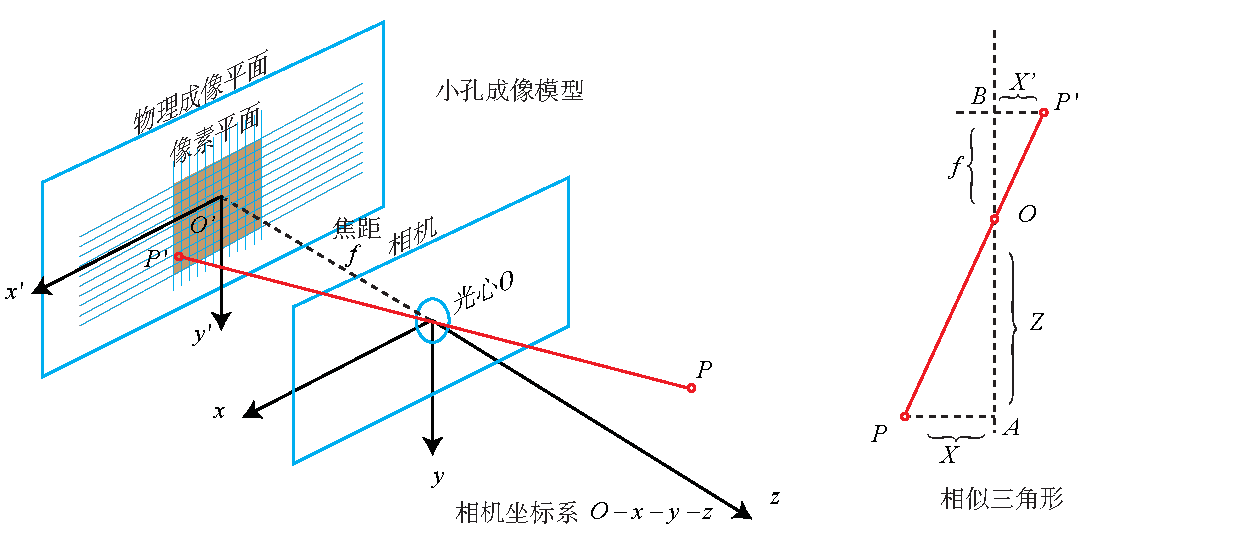
\includegraphics[width=1.0\textwidth]{chapter05/resources/cameraModel/cameraModel.pdf}
	\caption{Pinhole camera model. }
	\label{fig:cameraModel}
\end{figure}

Now geometrically model this simple pinhole model. Let $Oxyz$ be the camera coordinate system. It is customary for us to point the $z$ axis to the front of the camera, $x$ to the right, and $y$ to the down (this figure we should stand on the left side to see the right side). $O$ is the camera's \textbf{TODO}, which is also the pinhole in the pinhole model. The real world space point $P$, after being projected through the hole $O$, falls on the physical imaging plane $O'-x'-y'$, and the image point is $P'$. Let the coordinates of $P$ be $[X,Y,Z]^\mathrm{T}$, $P'$ is $[X',Y',Z']^\mathrm{T}$, and set the physics The distance from the imaging plane to the aperture is $f$ (focal length). Then, according to the similarity of triangles, there are:
\clearpage

\begin{equation}
\frac{Z}{f} = -\frac{X}{{X'}} =-\frac{Y}{{Y'}}.
\end{equation}

The negative sign indicates that the image is inverted. However, the image obtained by the actual camera is not an inverted image (otherwise the use of the camera would be very inconvenient). In order to make the model more realistic, we can equivalently place the imaging plane symmetrically in front of the camera, along with the 3D space points on the same side of the camera coordinate system, as shown by \autoref{fig:planes}. This can remove the negative sign in the formula to make the formula more concise:

\begin{equation}
\frac{Z}{f} = \frac{X}{{X'}} =\frac{Y}{{Y'}}.
\end{equation}

\begin{figure}[!htp]
	\centering
	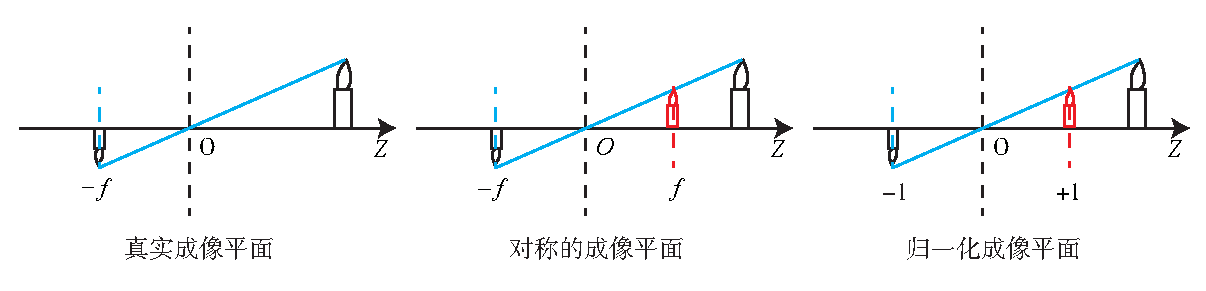
\includegraphics[width=1.0\textwidth]{chapter05/resources/cameraModel/planes.pdf}
	\caption{Real imaging plane, symmetrical imaging plane, normalized imaging plane.}
	\label{fig:planes}
\end{figure}

Put $X', Y'$ on the left side of the equation and sort it out:

\begin{equation}\label{eq:P2Pprime}
\begin{array}{l}
X' = f\frac{X}{Z}\\
Y' = f\frac{Y}{Z}
\end{array}.
\end{equation}

Readers may ask, why can we seem to move the imaging plane to the front at will? This is just the mathematical means we handle the real world and camera projection, and most of the images output by the camera are not inverted - the camera's own software will flip the image for you, so what we actually get is the symmetry, which is symmetrical The image on the imaging plane. So, although from the physical principle, the aperture imaging should be inverted, since we have pre-processed the image, it is understood that the image on the symmetry plane does not cause any harm. Therefore, without causing ambiguity, we do not limit the latter case to the pinhole model.

The formula \eqref{eq:P2Pprime} describes the spatial relationship between the point $P$ and its image, where the units of all points can be understood as meters, such as a focal length of 0.2 meters and $X'$ is 0.14 meters. However, in the camera, we end up with a single pixel, which also needs to sample and quantize the image on the imaging plane. To describe the process by which the sensor converts the perceived light into image pixels, we set a pixel plane $ouv$ on the physical imaging plane. We get \textbf{pixel coordinates} of $P'$ in the pixel plane: $[u,v]^\mathrm{T}$.

\textbf{pixel coordinate system}\footnote{ or image coordinate system, see section 2 of this lecture. } The usual way of definition is: the origin $o'$ is in the upper left corner of the image, the $u$ axis is parallel to the $x$ axis, and the $v$ axis is parallel to the $y$ axis. Between the pixel coordinate system and the imaging plane, there is a difference between \textbf{zoom} and a \textbf{translation of the origin}. We set the pixel coordinates to scale $\alpha$ times on the $u$ axis and $\beta$ times on $v$. At the same time, the origin is translated by $[c_x, c_y]^\mathrm{T}$. Then, the relationship between the coordinates of $P'$ and the pixel coordinate $[u,v]^\mathrm{T}$ is:

\begin{equation}
\label{eq:project2pixel1} 
\left\{
\begin{matrix} 
u=\alpha X' + c_x\\ 
v=\beta Y' + c_y
\end{matrix}
\right. .
\end{equation}

Substitute \eqref{eq:P2Pprime} and merge $\alpha f$ into $f_x$ and $\beta f$ into $f_y$ to get:

\begin{equation}
\left\{
\begin{matrix} 
u=f_x\frac{X}{Z} + c_x\\ 
v=f_y\frac{Y}{Z} + c_y
\end{matrix}
\right. .
\end{equation}

Among them, $f$ is in meters, $\alpha, and \beta$ is in pixels/meter, so $f_x, f_y$ and $c_x, c_y$ are in pixels. It would be more concise to write this form as a matrix, but the homogeneous coordinates are needed on the left and the non-homogeneous coordinates on the right:

\begin{equation}
\label{eq:intrinmatrix} 
\begin{pmatrix} u\\ v\\ 1 \end{pmatrix}=\frac{1}{Z}\begin{pmatrix} f_x & 0&c_x \\ 0& f_y& c_y\\ 0&0 & 1 \end{pmatrix}\begin{pmatrix} X\\ Y\\ Z \end{pmatrix} 
\buildrel \Delta \over =\frac{1}{Z} \bm{K} \bm{P}.
\end{equation}

In this equation, we refer to the matrix composed of the middle quantities as the camera's \textbf{inner parameter matrix} (Camera Intrinsics)$\bm{K}$. It is generally believed that the internal parameters of the camera are fixed after leaving the factory and will not change during use. Some camera manufacturers will tell you the internal parameters of the camera, and sometimes you need to determine the internal parameters of the camera, which is called \textbf{calibration}. In view of the maturity of the calibration algorithm (such as the famous single-player checkerboard Zhang Zhengyou calibration method \textsuperscript{\cite{Zhang1999}}), it will not be introduced here.

There are internal parameters, and naturally there are relative external parameters. Considering that in the formula ~\eqref{eq:intrinmatrix}~ we are using the coordinates of $P$ in the camera coordinate system. Since the camera is moving, the camera coordinates of $P$ should be the result of its world coordinates (denoted as $\bm{P}_w$) based on the current pose of the camera and converted to the camera coordinate system. The pose of the camera is described by its rotation matrix $\bm{R}$ and the translation vector $\bm{t}$. Then there are:

\begin{equation}
\label{eq:cameraprojection}
Z \bm{P}_{uv}=
Z \left[ \begin{array}{l}
u\\
v\\
1
\end{array} \right] = \bm{K} \left( {\bm{R}{ \bm{P}_w} + \bm{t}} \right) =  \bm{K} \bm{T} \bm{P}_w .
\end{equation}

Note that the latter formula implies a conversion from homogeneous to non-homogeneous coordinates (can you see it?)\footnote{ie, use homogeneous coordinates in $\bm{T}\bm{P}$ , then convert to non-homogeneous coordinates, and then multiply by $\bm{K}$. }. It describes the projection relationship of world coordinates to pixel coordinates of $P$. Among them, the camera's pose $\bm{R}, \bm{t}$ is also called the camera's \textbf{outside parameter} (Camera Extrinsics)\footnote{in robots or autonomous vehicles, the external reference is sometimes explained The transformation between the camera coordinate system and the robot body coordinate system, describing "where the camera is installed". }. Compared with the constant internal parameters, the external participation changes with the camera movement, and is also the target to be estimated in the SLAM, representing the trajectory of the robot.

The projection process can also be viewed from another perspective. The formula \eqref{eq:cameraprojection} shows that we can convert a world coordinate point to the camera coordinate system first, and then remove the value of its last dimension (that is, the depth of the point from the imaging plane of the camera), which is equivalent to the last One-dimensional \textbf{normalization processing}, get the projection of the point $P$ on the camera \textbf{normalized plane}:

\begin{equation}
\left( {\bm{R}{\bm{P}_w} + \bm{t}} \right) = \underbrace{\left[ X,Y,Z\right]^\mathrm{T}}_{\text{camera coordinates}} \to \underbrace {\left[ {X/Z,Y/Z,1} \right]^\mathrm{T}}_{\text{normalized coordinates}}.
\end{equation}

\textbf{normalized coordinates} can be seen as the front of the camera \footnote{Note that in the actual calculation, you need to check if $Z$ is positive, because the negative $Z$ can also get a point on the normalized plane by this method, but the camera will not capture the scene behind the imaging plane.} $z=1$ A point on the plane, this $z=1$ plane is also called \textbf{normalized plane}. Normalization coordinates and then multiplication of the inner parameters yield pixel coordinates, so we can consider the pixel coordinates $[u,v]^\mathrm{T}$ as the result of quantitative measurements on points on the normalized plane. It can also be seen from this model that if the camera coordinates are multiplied by any non-zero constant at the same time, the normalized coordinates are the same, which means that the depth of \textbf{point is lost during the projection process}, so the monocular The depth value of the pixel cannot be obtained in the visual.
